\chapter{Algorithm Design}
	\section{Requirements and Design Approach}
	
	Designing an efficient shortest-path algorithm requires balancing multiple factors, particularly accuracy, speed, and ease of implementation. To establish a clear framework, the algorithm must satisfy the following key properties:
	
	\begin{itemize}
		\item \textbf{Mathematical Correctness:} The algorithm must always return the true shortest path between the source and destination based on the given edge weights. No approximation should compromise the optimality of the result.
		\item \textbf{Computational Efficiency:} The algorithm should execute in a reasonable time frame, making it practical for large-scale graphs. A precise definition of "fast enough" is necessary to evaluate performance objectively.
		\item \textbf{Implementation Simplicity:} While complex optimizations can improve query speed, they often introduce additional implementation challenges. The chosen approach must balance efficiency with ease of development.
	\end{itemize}
	
	Among these properties, computational efficiency and implementation simplicity are in conflict. More sophisticated algorithms generally require intricate preprocessing steps or complex data structures, increasing implementation difficulty. Conversely, simpler algorithms may struggle with large graphs, leading to longer execution times.
	
	To make the problem more concrete, we define our primary objective as follows:
	
	\begin{quote}
		\textit{Find the shortest path from the Mathematics Department at SVNIT to Surat Railway Station within a subset of Surat’s road network (see Figure~\ref{fig:surat_graph}). The algorithm should match the path and approach the performance of NetworkX’s \texttt{shortest\_path} method.}
	\end{quote}

	\begin{figure}[h]
		\centering
		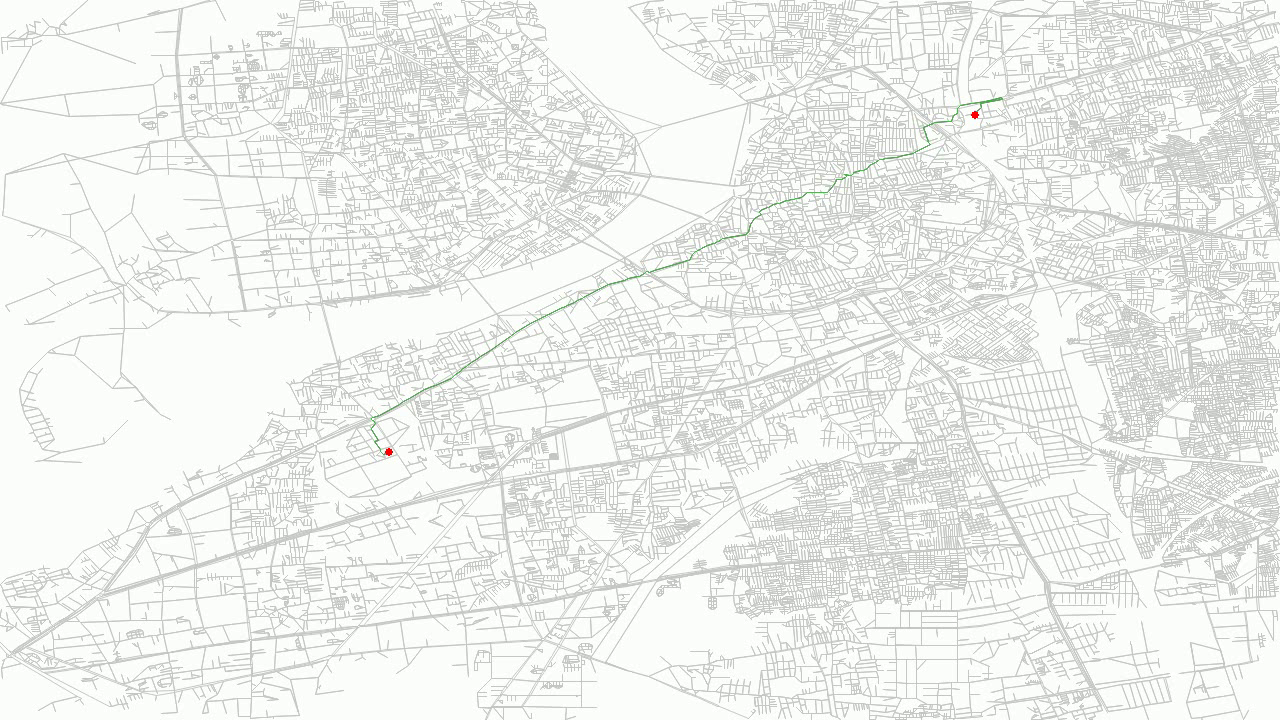
\includegraphics[width=1.0\textwidth]{surat_graph.png}
		\caption{Subset of Surat's road network used for pathfinding experiments.}
		\label{fig:surat_graph}
	\end{figure}

	This benchmark provides a measurable goal, allowing us to assess whether our solution is both computationally feasible and practically implementable. \newline
	
	To reconcile speed and simplicity, the algorithm was developed in successive iterations, gradually increasing complexity until achieving the desired performance. This stepwise approach enabled controlled performance improvements while maintaining clarity in implementation.\newline
	
	To facilitate this process, we have developed a tool that measures execution time and provides a visual representation of the computed paths. This tool enables direct comparisons between different algorithmic approaches, helping us refine our implementation to reach the desired performance, as well as roughly evaluate the correctness of our algorithm.
	
	\section{Version 1: Basic Dijkstra's Algorithm}
	
	The first version of our algorithm is based on \textbf{Dijkstra's shortest-path algorithm}, a classical approach for computing the optimal path in a weighted graph with non-negative edge weights.
	
	\subsection{Performance and Limitations}
	
	To evaluate the performance of this implementation, we measured its execution time using the visualization tool developed for this project (see Figure~\ref{fig:dijkstra_timing}).
	
	\begin{figure}[h]
		\centering
		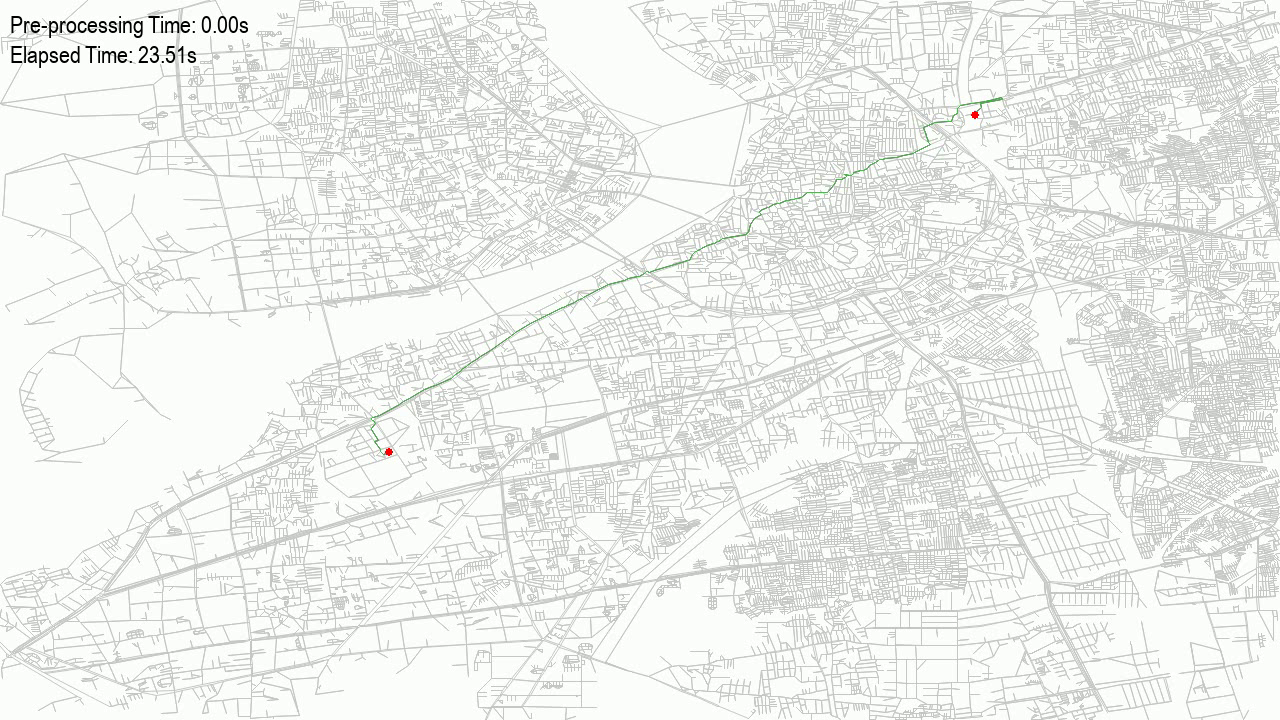
\includegraphics[width=1.0\textwidth]{dijkstra.png}
		\caption{Visualization of the execution time for Version 1.}
		\label{fig:dijkstra_timing}
	\end{figure}
	
	While this version is a reliable starting point, it has several limitations:
	\begin{itemize}
		\item It explores nodes in an uninformed manner, leading to inefficiencies.
		\item Query times can be slow for large graphs due to excessive node expansion.
		\item No preprocessing is used, making repeated queries inefficient.
	\end{itemize}
	
	\section{Version 2: A* Search Algorithm}
	
	The second version of our algorithm introduces the \textbf{A* search algorithm}, an improvement over Dijkstra's algorithm that incorporates heuristic guidance to prioritize more promising paths.
	
	\subsection{Performance and Limitations}
	
	To evaluate the efficiency of A*, we measured its execution time using the visualization tool developed for this project (see Figure~\ref{fig:astar_timing}).
	
	\begin{figure}[h]
		\centering
		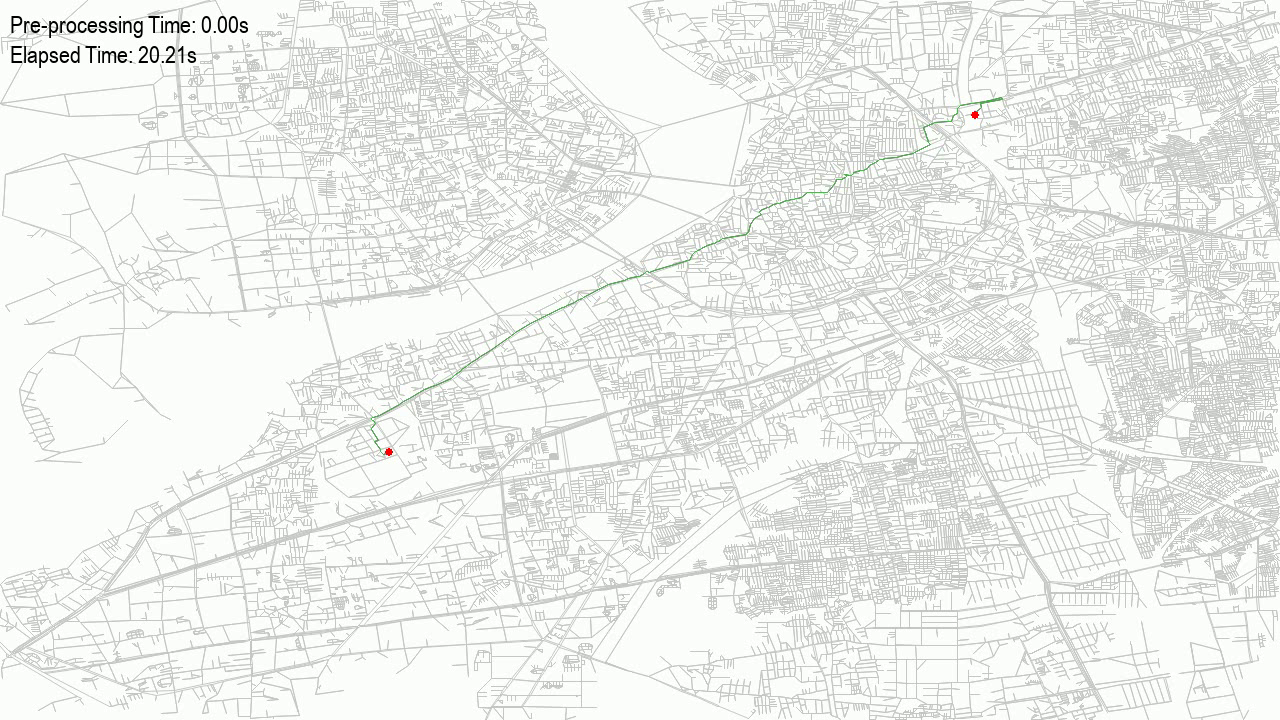
\includegraphics[width=1.0\textwidth]{astar.png}
		\caption{Visualization of the execution time for Version 2.}
		\label{fig:astar_timing}
	\end{figure}
	
	While A* significantly improves upon Dijkstra’s algorithm by reducing unnecessary node expansions, it has certain limitations:
	\begin{itemize}
		\item The efficiency of A* heavily depends on the quality of the heuristic function.
		\item In some cases, particularly when the heuristic is weak or misleading, A* may perform similarly to Dijkstra’s algorithm.
		\item Like Dijkstra's algorithm, A* does not leverage preprocessing, making repeated queries inefficient.
	\end{itemize}
	
	Despite these limitations, A* provides a substantial improvement in query speed and forms the basis for further optimizations in later versions.
	
	\section{Version 3: Bidirectional Dijkstra's Algorithm}
	
	The third version of our algorithm improves upon Dijkstra’s algorithm by introducing \textbf{bidirectional search}, which simultaneously expands paths from both the start and the destination. This significantly reduces the number of nodes explored, improving efficiency.
	
	\subsection{Performance and Limitations}
	
	To analyze its efficiency, we measured the execution time of this version using our visualization tool (see Figure~\ref{fig:bidirectional_timing}).
	
	\begin{figure}[h]
		\centering
		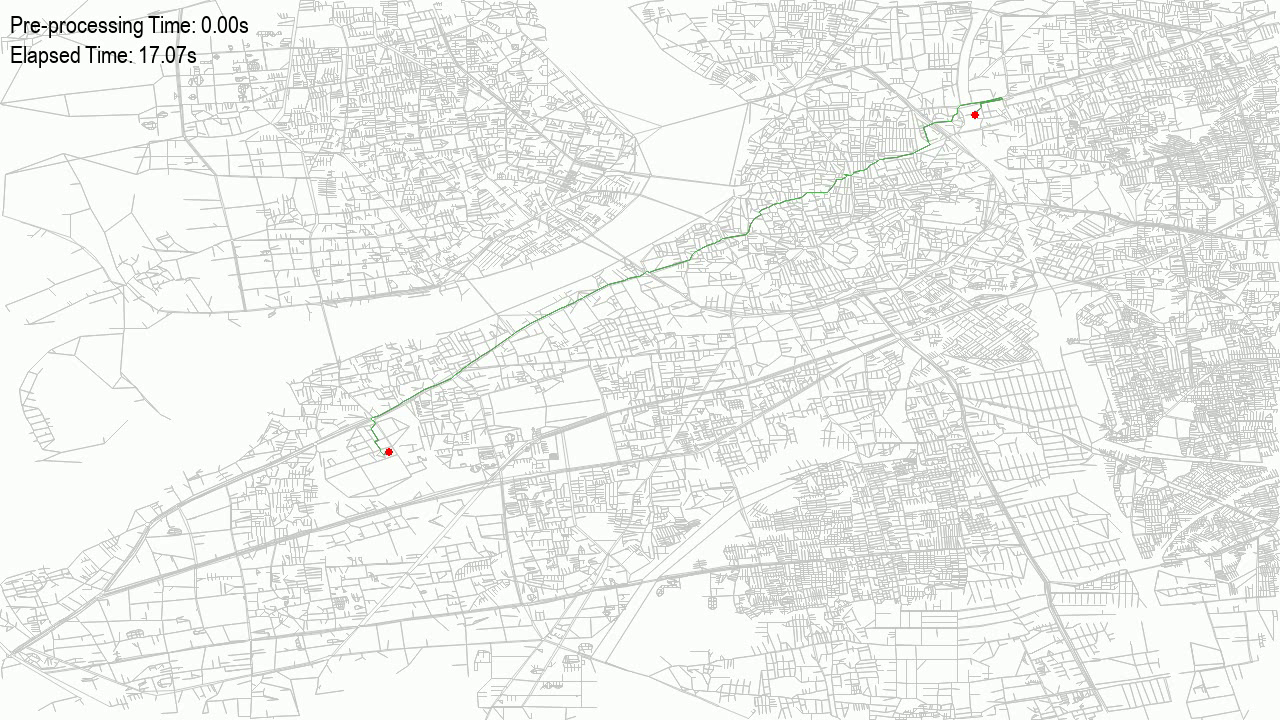
\includegraphics[width=1.0\textwidth]{bidirectional_dijkstra.png}
		\caption{Visualization of the execution time for Version 3.}
		\label{fig:bidirectional_timing}
	\end{figure}
	
	While bidirectional search provides significant speed improvements over standard Dijkstra’s algorithm, it has some limitations:
	\begin{itemize}
		\item It requires additional data structures to maintain two search frontiers.
		\item Performance gains depend on how quickly the two searches meet; in some cases, improvement over A* may be marginal.
		\item Like previous versions, it does not use preprocessing, making repeated queries inefficient.
	\end{itemize}
	
	Despite these limitations, bidirectional search is a key optimization that brings us closer to an efficient pathfinding solution.
	
	\section{Version 4: Bidirectional A* Search Algorithm}
	
	The fourth version of our algorithm combines the optimizations of \textbf{A* search} with the efficiency of \textbf{bidirectional search}. By guiding both forward and backward searches using heuristic estimates, Bidirectional A* significantly reduces the number of expanded nodes, further improving query speed.
	
	\subsection{Performance and Limitations}
	
	We evaluated the execution time of this version using our visualization tool (see Figure~\ref{fig:bidirectional_astar_timing}).
	
	\begin{figure}[h]
		\centering
		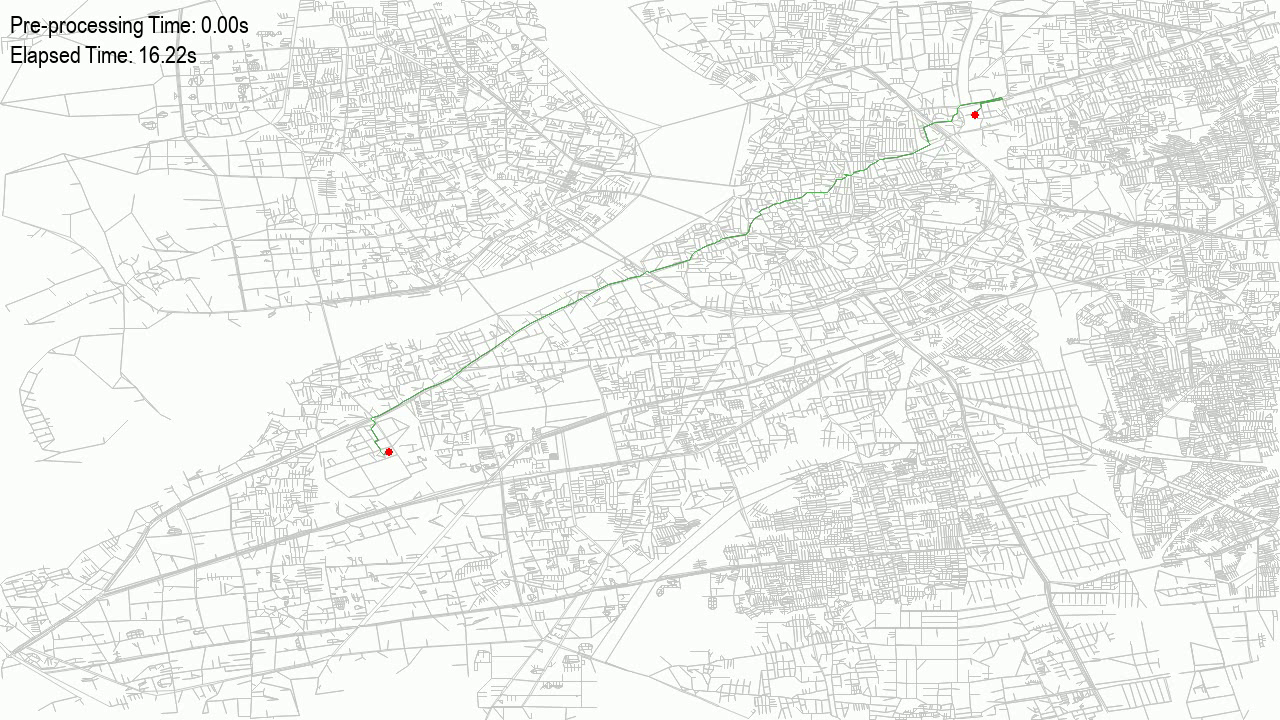
\includegraphics[width=1.0\textwidth]{bidirectional_astar.png}
		\caption{Visualization of the execution time for Version 4.}
		\label{fig:bidirectional_astar_timing}
	\end{figure}
	
	While Bidirectional A* improves upon previous versions, it has some limitations:
	\begin{itemize}
		\item Performance heavily depends on the accuracy of the heuristic function.
		\item If the heuristic is weak or inconsistent, the speed gains over Bidirectional Dijkstra may be minimal.
		\item The implementation is more complex due to managing two synchronized A* searches.
	\end{itemize}
	
	Despite these challenges, Bidirectional A* provides a significant improvement in pathfinding efficiency and forms the basis for even more advanced optimizations.
	
	\section{Version 5: Bidirectional A* Search with ALT Preprocessing}
	
	The final version of our algorithm incorporates preprocessing techniques to further enhance efficiency. By integrating \textbf{A* search}, \textbf{bidirectional search}, and \textbf{ALT preprocessing}, this version achieves significant improvements in query speed while maintaining accuracy.

	\subsection{Performance and Limitations}
	
	We evaluated the execution time of this version using our visualization tool (see Figure~\ref{fig:bidirectional_alt_timing}).
	
	\begin{figure}[h]
		\centering
		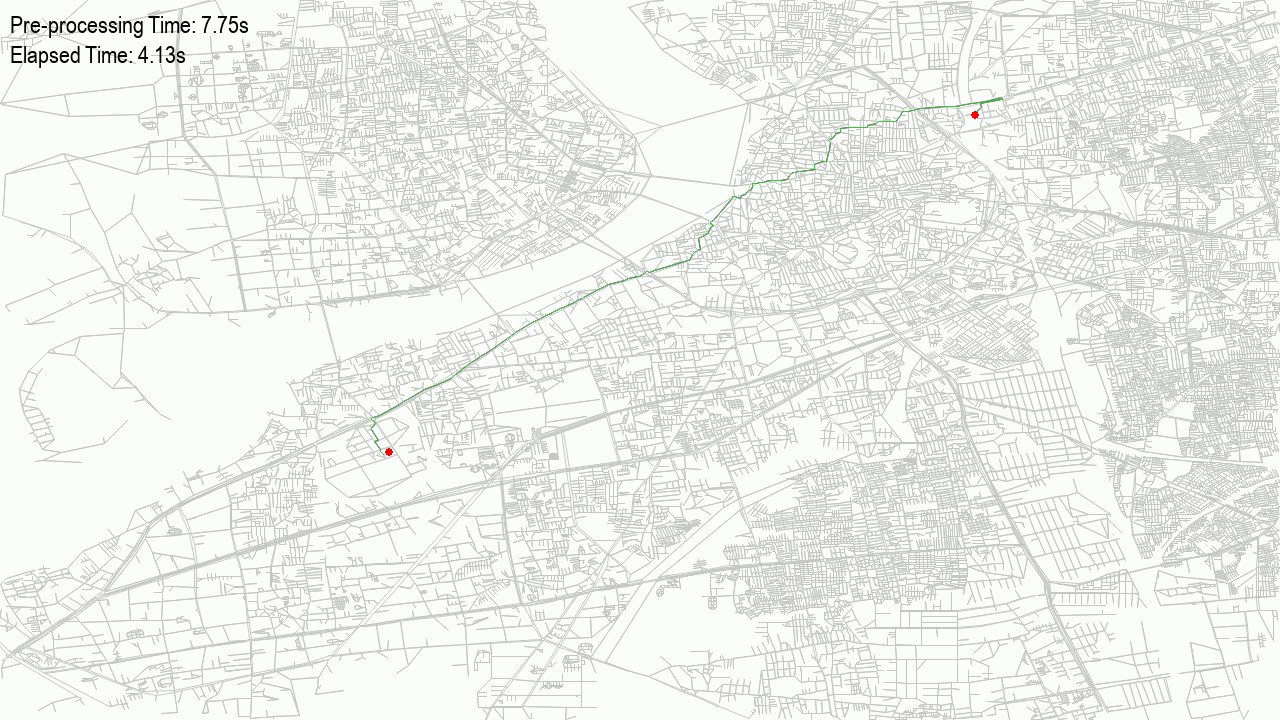
\includegraphics[width=1.0\textwidth]{final.png}
		\caption{Visualization of the execution time for Version 5.}
		\label{fig:bidirectional_alt_timing}
	\end{figure}
	
	This version achieves significant speed improvements but comes with trade-offs:
	\begin{itemize}
		\item The initial computation of landmark distances requires additional processing time.
		\item Storing shortest paths for multiple landmarks increases space complexity.
		\item If the graph changes dynamically (e.g., road closures), the preprocessing must be updated.
	\end{itemize}
	
	Despite these challenges, this final version represents the most optimized solution developed in this project, balancing preprocessing efficiency with rapid query execution. \newline
	
	The code for the final algorithm can be referred to at \textbf{Appendix \ref{appendix:design:final_code}}.